\newpage

\section{Metode og Proces}
I nedstående afsnit fremlægges metoder og processer brugt til udviklingen af
Dungeons and Gnoblins spillet.

\subsubsection{Gruppedannelse}
Gruppen blev dannet på baggrund af at vi som studerende selv skulle finde medlemmer og danne projektgrupper. 4 af gruppens medlemmer havde tidligere arbejdet sammen om et semesterprojekt, hvor samarbejdet var godt nok til at danne gruppe igen. De 4 af gruppens medlemmere var dermed dannet inden semesterets start og de resterende 4 blev indmeldt efter offentliggørelsen af semesterprojektet. Der var i gruppensdannelse ikke taget hensyn til personlighedsprofiler, men mere bare dannet efter første-til-mølle-princip på baggrund af et opslag. Gruppen redegjorde først ideer til projektet og blev hurtigt forventningsafstemt om projektets resultat skulle være middelmådigt. 

\subsubsection{Projektforløb, SCRUM og møder}
Projektets endelige mål har været implementeringen af et text-based adventure game.
Hertil har gruppen gjort brug af agile processen til at imødekomme dette mål.

Først har gruppen specifiseret Kravspecifikationerne for spillet, med ønsker om
hvilke features spillet har skulle inkludere. Continuous integration er dernæst
været et vigtigt værktøj til implementeringen af de ønskede features, med et klart
ønske om at integrere nye features ind i projektet få tidligt som muligt.\\

I løbet af projektforløbet blev der afholdt to faste ugentlige møder. Et internt gruppemøde om mandagen og vejledermøde om onsdagen. Hertil var der fra start uddelt rollerne Mødeleder og referent til gruppens medlemmer som gik på skift hver uge. Til hvert møde blev der gennemgået hvad der var blev arbejdet med, hvilke udfordringer der forekom samt hvad der fremadrettet skulle arbejdes med for hver af gruppens medlemmer. Dette gjorde vi i form af SCRUM for at give et bedre overblik for projektets fremgang og dermed vurderer om gruppen var bagud eller foran ift. Gruppens tidsplan. Vores SCRUM-proces var ikke avanceret hvor der blev koordineret SCRUM Master og Product Owner, men blev derimod anvendt som redskab til at skabe et overblik over arbejdsfordelingen og udviklingen. Tidsplanen blev udarbejdet ved projektets start og havde formålet at give gruppen deadlines for projektets udviklingsproces. 

Det interne møde om mandagen var struktureret så der først på mødet blev diskuteret om hvilke arbejdsopgaver der var blevet færdiggjort fra hvert modul. Hvis der var noget der skulle præsenteres overfor de andre medlemmer, blev det vist her. Efterfølgende blev der forddelt arbejdsopgaver ud til hver af gruppens medlemmer. Når dagsordenen var færdig, gik gruppen derefter igang med at arbejde på deres forskellige opgaver. De opgaver der blev tilddelt havde typisk en arbejdsbyrde i det omfang at det kunne færdiggøres indenfor to dage, så det kunne vises til vejledermøde onsdag. Herunder ses et eksempel på hvordan gruppens mødeindkaldelse ser ud.

\begin{figure}[H]
  \centering
  \includegraphics[scale=.5]{02-Body/Images/Mødeindkaldelse-eksempel.png}
  \caption{Viser et billed af hvordan gruppen indkaldte til møder og hvordan dagsordenen blev sat inden mødet. Her kan det også udleddes at hvert modul præsenterede deres arbejde i løbet af mødet. Derudover ses der også liste af mødeledere de forskellige uger.
  \label{fig:Agile}
\end{figure}

\begin{figure}[H]
  \centering
  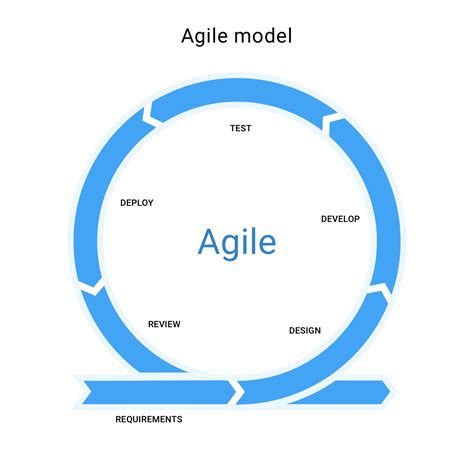
\includegraphics[scale=.5]{02-Body/Images/Agile.png}
  \caption{Viser et billed af agile modellen som består af mangle iterationer
           af design, develop, test, og deploy. Dette minder om continuous integration
           og har hindret mange problemmer for udviklingsforløbet}
  \label{fig:Agile}
\end{figure}

SCRUM og AGILE bringer klarhed til medlemmerne om deres roller og opgaver over en 
kommende tidperiode med en backlog over opgaver, som skal færdiggøres over et sprint (1 uge).
Ugentlige opdateringer og møder omkring potentielle problemmer udviklingsforløbet betyder
at gruppen har kunne tage hånd om evt. problemmer tidligt i forløbet og derved løse dem
før de har udviklet sig til større problemmer.

Til styring og implementering af souce code har vi benytte git som et version control system.
fordelen ved git er at det tillade flere udviklere at arbejde på det samme projekt og integere 
deres løsninger. Der er dog chancer for merge konflikter hvilket kan, i værkste tilfælde, før
til problemmer med at integrer de forskellige løsninger korrekt med hinanden.

\subsubsection{Konflikthåndtering og samarbejdskontrakt}
Gruppen gjorde det klart ved dannelsen at dette er et gruppeprojekt og at alle medlemmere havde en kritisk rolle for projektet. Derfor blev der skabt et fundament over at præstationen for hvert medlem skulle være tilstrækkelig. Hvis der skulle opstå udfordringer i løbet af arbejdsopgave skulle dette kommunikkeres ud, så der i fællesskab kunne findes en løsning. I gruppens samarbejdskontrakt blev det også pointeret at hvis der skulle opstå en konflikt mellem gruppens medlemmere, ville dette løses i fællesskab med de resterende medlemmere af gruppen. For dette projekt forekom der ikke nogen konflikter mellem gruppens medlemmer og samarbejdet har været suverænt gennem hele projektet. Uenigheder omkring projektet blev også taget op med vejleder, hvilket blev brugt til at gøre ting mere klart omkring hvilke løsninger ville være optimalt i den givne situation. 

\subsubsection{Arbejdsfordeling}
I et tidligt stadie i projektet blev arbejdet fordelt mellem gruppens medlemmer i form af systemets moduler. Efter en beslutning af hvilke moduler der skulle være i systemet, blev der fordelt 2 medlemmer på hver af de 4 moduller(Front-End, Game Logic, Back-End og Database. Der blev sat 2 personer på hvert modul, så medlemmerne kunne rådgive og samarbejde om modulet. Dermed ville der ikke være et medlem som var alene om et modul. Medlemmerne ønskede hvad de foretrak at arbejde med og dermed blev der fordelt ud fra de ønsker. Fra starten af var der usikkerhed om arbejdsbyrden på de forskellige moduler, da det var tidligt på semesteret og der ikke var kommet så mange lektioner i de forskellige fag. Dermed valgte vi fordele det på baggrund af interesse fremfor forhåndsviden, da interesse kunne fremme arbejdsmentaliteten. 

\subsubsection{Projektadminstration}
Al kommunikation mellem gruppens medlemmer foregik på Messenger eller discord. Det er også her at gruppen gav besked om hvornår der var møder og om der blev sendt besked til vejleder om referat til onsdagens vejledermøder. I det tidlige stadie blev der også bestemt hvilke redskaber der skulle anvendes i løbet af projektet. Et fælles repository blev oprettet på Github hvor projektets filer kunne lagres, så alle havde adgang til dem. På Github var gruppens taskboard også oprettet hvor gruppen kunne se hvilke opgaver der skulle gennemføres. Der kan dog i retrospektiv siges at taskboardet ikke blev opdateret ofte, da gruppens medlemmer havde et godt overblik over deres egne opgaver efter gruppemøder om mandagen. Redskaberne til SCRUM såsom backlog, sprint retrospective, spring review og burndowncharts blev ikke anvendt, da vi ikke fandt det relevant i projektets udvikling.  

\subsection{Modellering}
Projektet benytter UML til at beskrive og modellere software-- arkitektur
og design, hvilket gør det nemt at simplificere og visualisere strukturen på software
løsningen. 

Selve arkitekturen er vist med C4 modellen som giver et lageret indblik i både
akitekturen på et højt niveau, men med evnen til at give en detaljeret beskrivelse
af systemmets komponenter og deres kommunikation med hinanden.

\begin{figure}[H]
  \centering
  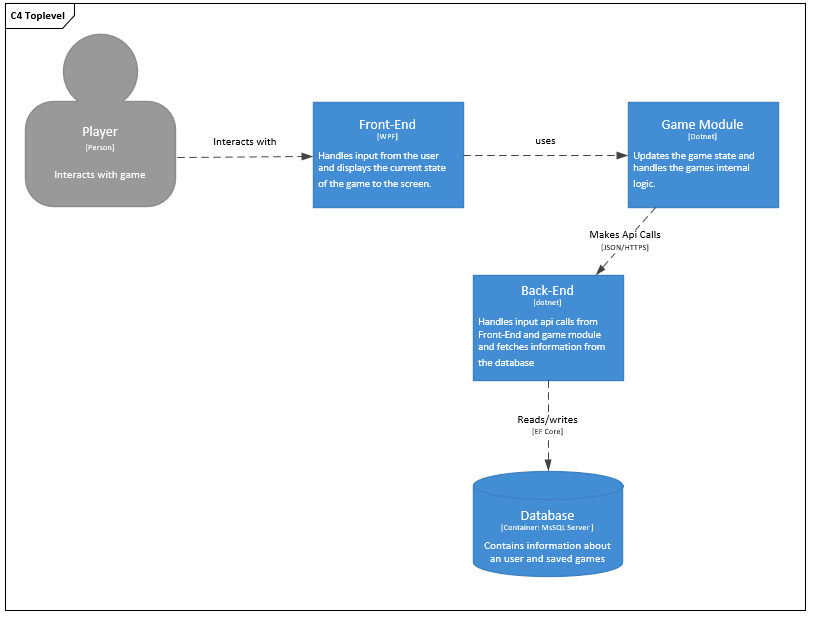
\includegraphics[scale=0.8]{02-Body/Images/C4TopLvlDB.PNG}
  \caption{}
  \label{fig:c4}
\end{figure}

STM og SD diagrammer er brugt til at give programmets udførsel struktur, og fungere
som en hjælp til at visualisere programmets forskellige states og flow of execution.
Det giver et nemt overblik over hvordan funktionskald mellem forskellige komponenter
har skal fungere således, at der ikke opstår misforsåelse grupperne imellem. 

Generelt er arkitekturen opbygget som "pseudo" diagrammer. Dvs. de ligner ikke fuldstændigt 
det endelige design, men har til formål at vise den overordnede tankegang i systemet og 
samtidig virke som et udviklingsværktøj til at videreudvikle systemet. Da der i gruppen 
er blevet arbejdet iterativt, er der forskelle mellem diagrammer for arkitektur og design,
da der er blevet tilføjet flere moduler og funktioner undervejs. Den overordnede tanke i 
projektet er der dog ikke blevet ændret på.

\subsubsection{Iterativ Udviklingsforløb}

AGILE og continuous integration fungerer på en naturlig iterativ måde, der tillader 
ændringer til måde designet og implementeringen undervejs i udviklingsforløbet.
Under hvert SCRUM møde er der taget stilling til om, der skulle laves ændringer i 
gruppens tilgang til projektet, altså om en implementering skulle ændres. \\

Et eksempel har været kommunikationen mellem Game Engine og Frontend, hvor frontend
har haft svært ved at håndtere komplicered return types. Der er sålede lavet
ændringer for at gøre det nemmere for frontend at udnytte den infomation som Game Engine
har returneret efter et funktionskald.

Denne flexible arbejdsmetode har igen ført til at problemmer ikke har kunne vokse men
at der blevet taget hånd om dem mens det stadig har været muligt at håndtere dem.
Overordnet set har vi ligesom de tidligere 

\subsection{Konklusion på projektets proces}
Processen for dette semester har været anderledes sammenlignet med de forrige semesterprojekter for gruppen. Da der i dette semester kun var fokus software, skulle der anvendes en anden model for klargørelse af projektets arkitektur. Da 4 af gruppens medlemmere havde arbejdet sammen før i tidligere projekter, blev der hurtigt sat en 'skabelon' for hvordan gruppen skulle arbejde. Der er generelt ikke tænkt meget over hvordan projekts proces skulle være undervejs i projektet, men i retrospektiv har denne opbygning af projektets proces været den mest optimale for gruppen og har været med til at bringe det bedste frem i alle af gruppens medlemmere. Som konklusion er der blevet lagt vægt på samarbejde og at gruppens udfordringer blev løst bedst sammen. På baggrund af de næsten ikke-eksisterende konflikter, har der ikke hersket tvivl om hvordan gruppen skulle arbejde og dermed har processen næsten allerede givet, da gruppen blev dannet.
